\documentclass[final]{article}
\usepackage[paperwidth=24in,paperheight=36in,margin=1in]{geometry}
\usepackage{tikz}
\usetikzlibrary{shapes,arrows.meta,positioning,fit}

\pagestyle{empty}

\begin{document}

\begin{center}
{\Huge \textbf{FATE’S EDGE — SYSTEMS CONNECTION MAP}}\\[0.5em]
{\Large Mechanics serve narrative. Narrative feeds choice.}
\end{center}

\vspace{1em}

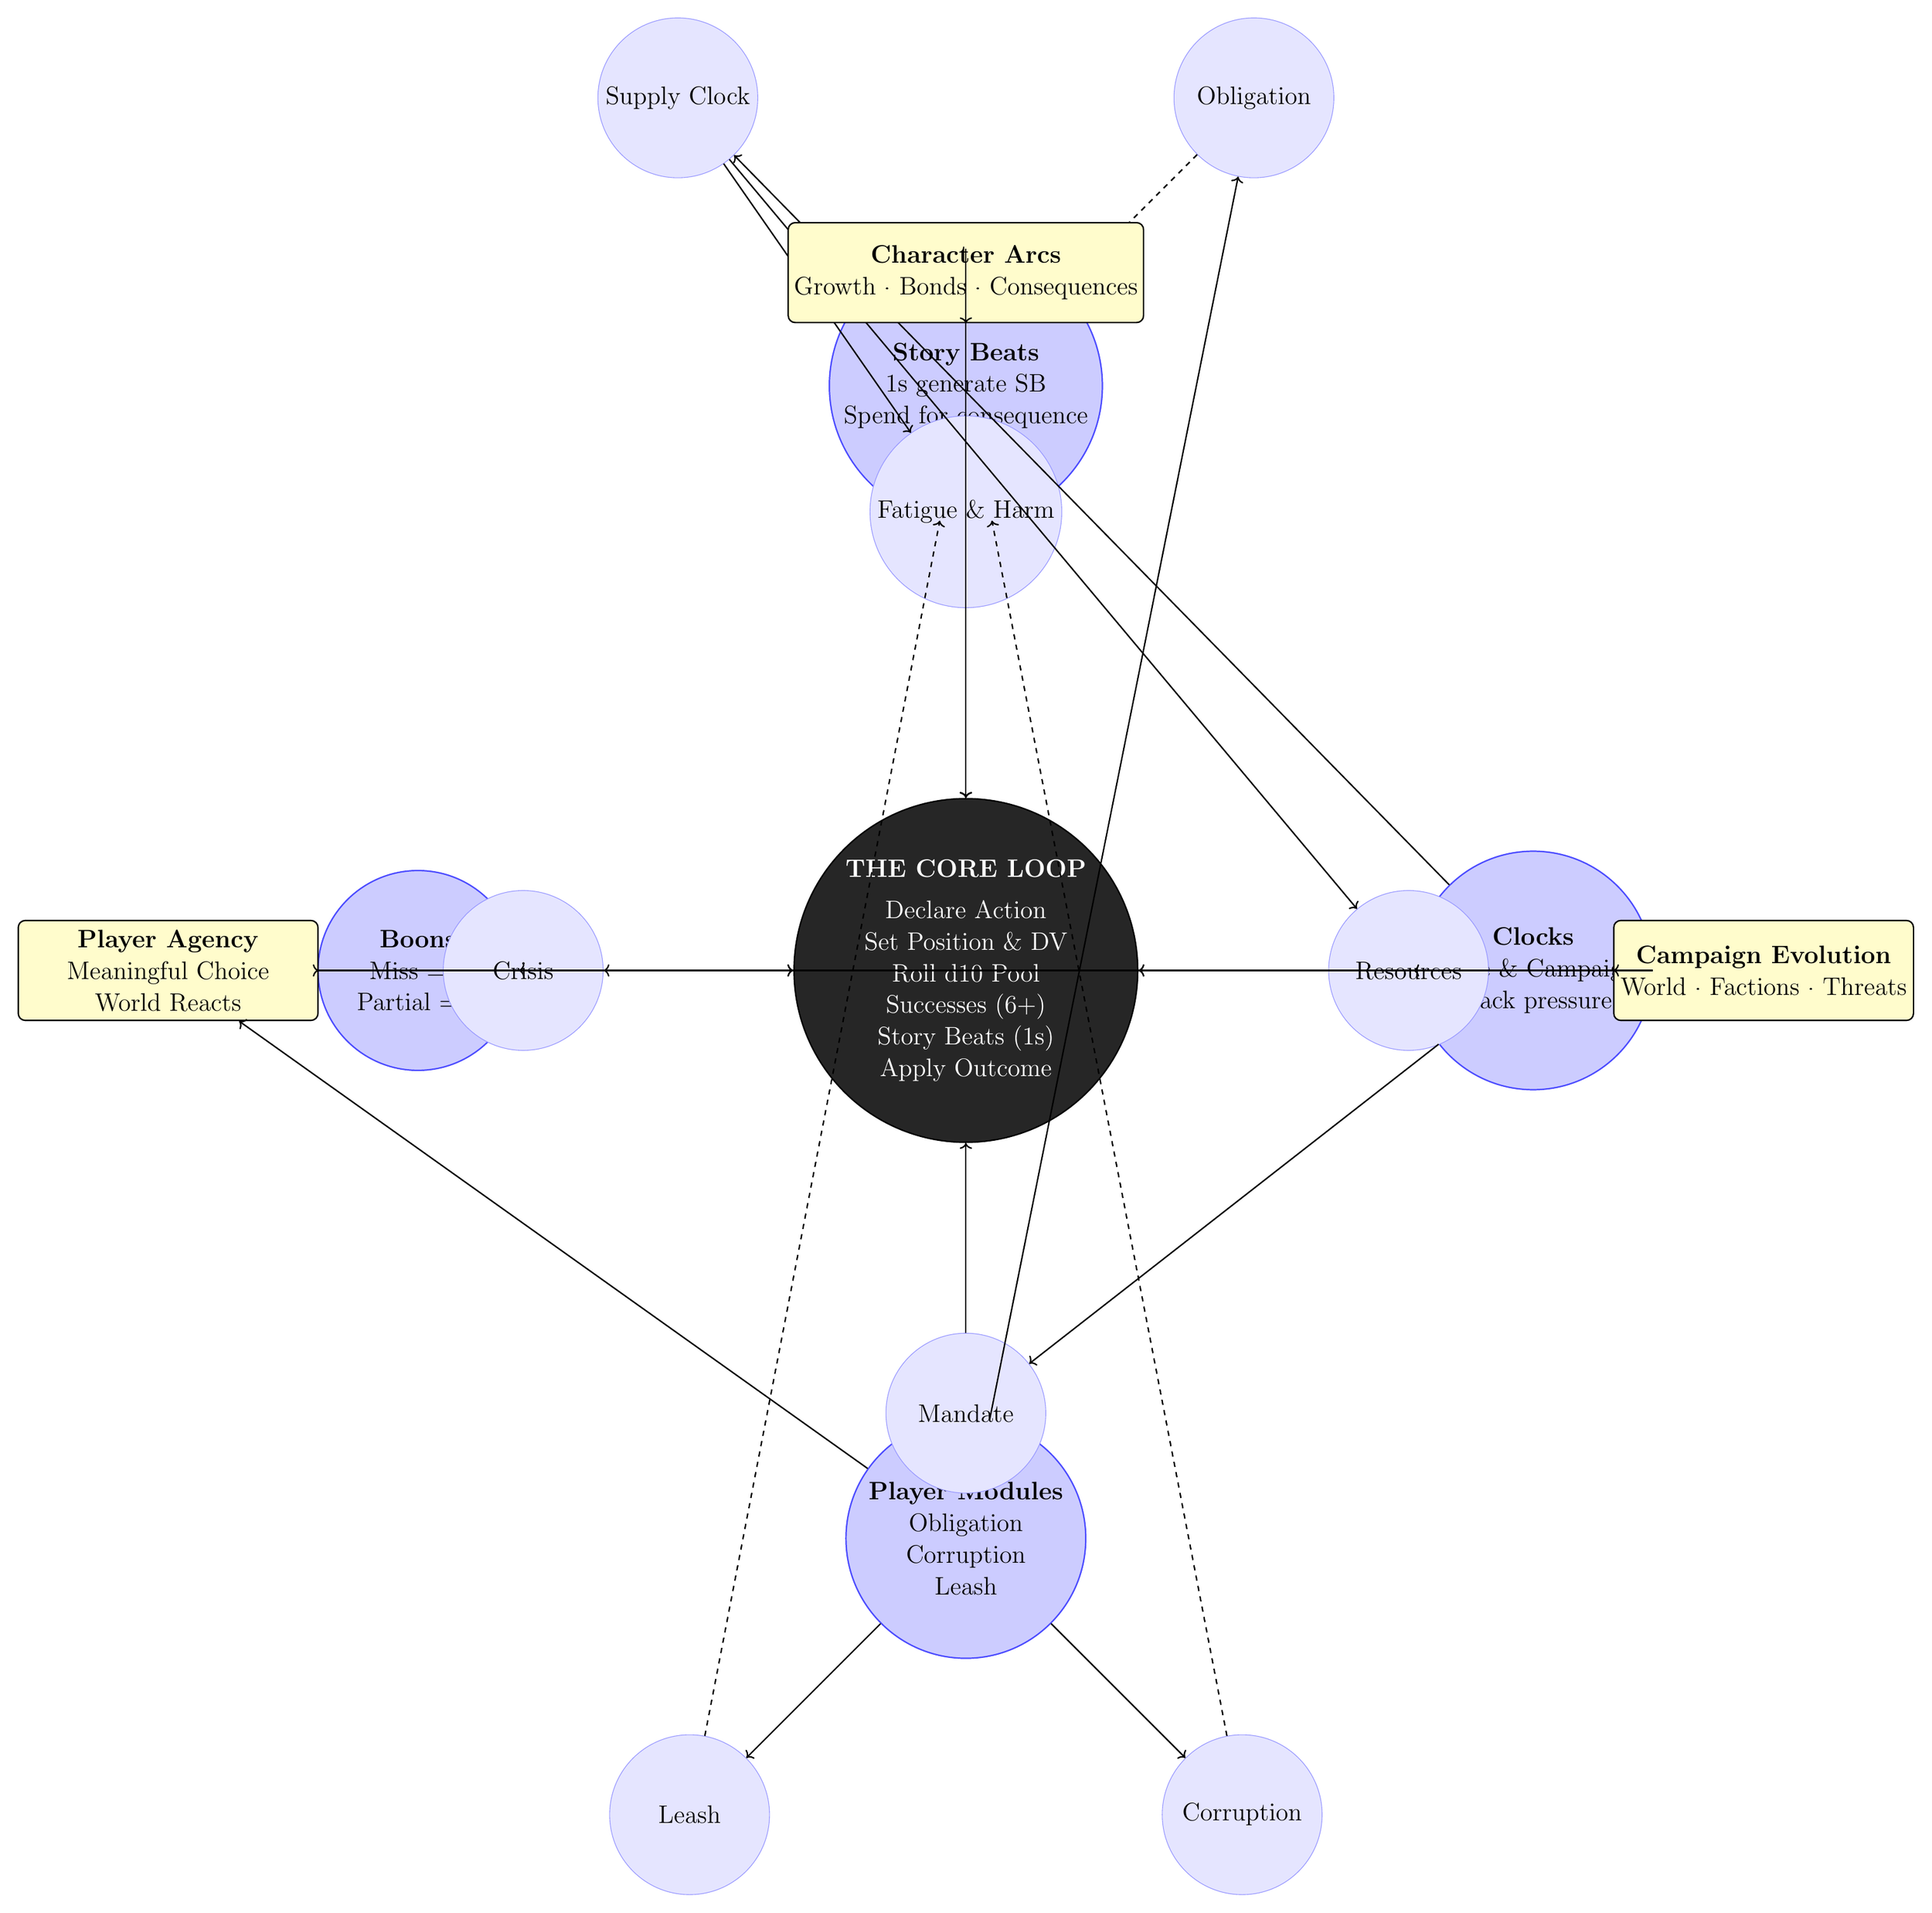
\begin{tikzpicture}[
    node distance=2.5cm,
    every node/.style={align=center,font=\Large},
    core/.style={circle,draw=black,fill=black!85,text=white,thick,minimum size=5cm},
    primary/.style={circle,draw=blue!70,fill=blue!20,thick,minimum size=4cm},
    secondary/.style={circle,draw=blue!40,fill=blue!10,minimum size=3.2cm},
    narrative/.style={rectangle,rounded corners,draw=black,fill=yellow!20,thick,minimum width=6cm,minimum height=2cm},
    arrow/.style={->,thick},
    dottedarrow/.style={->,thick,dashed}
]

% =====================
% CORE
% =====================
\node[core] (core) {
\textbf{THE CORE LOOP}\\[0.4em]
Declare Action\\
Set Position \& DV\\
Roll d10 Pool\\
Successes (6+)\\
Story Beats (1s)\\
Apply Outcome
};

% =====================
% FIRST RING
% =====================
\node[primary,above=5.5cm of core] (sb) {
\textbf{Story Beats}\\
1s generate SB\\
Spend for consequence
};

\node[primary,right=5.5cm of core] (clocks) {
\textbf{Clocks}\\
Scene \& Campaign\\
Track pressure
};

\node[primary,below=5.5cm of core] (modules) {
\textbf{Player Modules}\\
Obligation\\
Corruption\\
Leash
};

\node[primary,left=5.5cm of core] (boons) {
\textbf{Boons}\\
Miss = 2\\
Partial = 1
};

% Core connections
\draw[arrow] (core) -- (sb);
\draw[arrow] (core) -- (clocks);
\draw[arrow] (core) -- (modules);
\draw[arrow] (core) -- (boons);

\draw[arrow] (sb) -- (core);
\draw[arrow] (clocks) -- (core);
\draw[arrow] (modules) -- (core);
\draw[arrow] (boons) -- (core);

% =====================
% SECOND RING
% =====================
\node[secondary,above right=3.8cm of sb] (obligation) {Obligation};
\node[secondary,below right=3.8cm of modules] (corruption) {Corruption};
\node[secondary,below left=3.8cm of modules] (leash) {Leash};
\node[secondary,above left=3.8cm of sb] (supply) {Supply Clock};

\node[secondary,above=3.8cm of core] (fatigue) {Fatigue \& Harm};
\node[secondary,right=3.8cm of core] (resources) {Resources};
\node[secondary,below=3.8cm of core] (mandate) {Mandate};
\node[secondary,left=3.8cm of core] (crisis) {Crisis};

% Second-ring arrows
\draw[arrow] (modules) -- (obligation);
\draw[arrow] (modules) -- (corruption);
\draw[arrow] (modules) -- (leash);

\draw[arrow] (clocks) -- (supply);
\draw[arrow] (clocks) -- (mandate);
\draw[arrow] (clocks) -- (crisis);

\draw[arrow] (supply) -- (fatigue);
\draw[arrow] (supply) -- (resources);

\draw[arrow] (resources) -- (boons);
\draw[arrow] (resources) -- (clocks);

\draw[dottedarrow] (obligation) -- (sb);
\draw[dottedarrow] (corruption) -- (sb);
\draw[dottedarrow] (leash) -- (sb);

\draw[arrow] (fatigue) -- (core);

% =====================
% NARRATIVE RING
% =====================
\node[narrative,above=9.5cm of core] (character) {
\textbf{Character Arcs}\\
Growth · Bonds · Consequences
};

\node[narrative,right=9.5cm of core] (campaign) {
\textbf{Campaign Evolution}\\
World · Factions · Threats
};

\node[narrative,left=9.5cm of core] (agency) {
\textbf{Player Agency}\\
Meaningful Choice\\
World Reacts
};

\draw[arrow] (sb) -- (character);
\draw[arrow] (clocks) -- (campaign);
\draw[arrow] (modules) -- (agency);
\draw[arrow] (boons) -- (agency);

\draw[arrow] (character) -- (core);
\draw[arrow] (campaign) -- (core);
\draw[arrow] (agency) -- (core);

\end{tikzpicture}

\vfill
\begin{center}
\Large
\textit{Always start with fiction. Add only one new system per scene.}\\
\textbf{SB Budget = 4 + Tier \quad | \quad Max 3 active clocks per scene}
\end{center}

\end{document}